%!TEX root = ../Studienarbeit.tex

\chapter{Umsetzung}

\section{Softwareentwicklung}
In diesen Abschnitt werden einige Kernkomponenten der Software detaillierter dargestellt und die Auswahl des Mikrocontrollers beschrieben.

\subsection{Auswahl der Mikrocontrollers}
Als Mikrocontroller wird das ESP32-WROOM-32E-Modul verwendet. Dies hat mehrere Gründe, welche nachfolgend zu finden sind.
Als erster Grund, welcher für die Verwendung des ESP32 spricht, ist die große Beliebtheit des Mikrocontrollers in Hobbyprojekten und daraus folgernd eine große Community die bei Problemen in der Entwicklung unterstützen kann \cites{redditESP32}{esp32Forum}. Ebenfalls ist eine gute Dokumentation der \ac{ESP-IDF} durch Kommentare im Sourcecode, sowie durch Beispielprogramme gegeben. Als weiterer Grund für die Verwendung des ESP32 spricht, die Unterstützung mehrerer Bluetooth-Stacks, welche in Kapitel \ref{section:bluetoothStacks} beschrieben sind. Als letzter Grund ist noch die Verfügbarkeit der Mikrocontroller in kompakten Hardwaremodulen, in denen alle benötigen Hauptkomponenten für den Betrieb des Mikrocontrollers enthalten sind, wie Kondensatoren, Widerständen und in manchen Modulen ebenso die benötigte Antenne für den Betrieb von Bluetooth oder \acs{WLAN} \cite[S.~14]{espressifHardwareDesignGuidelines}. Auch haben die ESP32-Module meist eine CE-Zertifizierung, wie in Kapitel \ref{section:esp32Explained} beschrieben ist und dadurch könnte das entwickelte Fernsteuerungsmodul vereinfacht für den Vertrieb zertifiziert werden. Trotz den vorhandenen Funktionsumfang und Ökosystem ist das ESP32-Modul kostengünstig und im Bereich um 5~€ zu erwerben \cite{espressifModules}.

\subsection{Auswahl des Bluetooth-Stacks}
Als Bluetooth-Stack für den ESP32 wird der Open Source \ac{BLE}-Stack Apache NimBLE verwendet. Dies hat den Hintergrund, dass die Kommunikation ausschließlich zwischen dem Fernsteuerungserweiterungsmodul und Endgeräten mittels \ac{BLE} erfolgen soll. Für diesen Einsatzzweck wird die Verwendung von Apache NimbLE empfohlen, da dieser kompakter in der Codegröße ist und weniger Speicher zur Laufzeit benötigt \cite{espidfBluetoothStack}.

\subsection{Kommunikation zwischen dem Mikrocontroller und dem Endgerät}
\label{section:communicationModuleDevice}
Für die Übermittlung der Daten zwischen dem Mikrocontroller zu einem Endgerät wird \ac{BLE} verwendet, indem die Fernsteuerungsdaten mittels \ac{HOGP} verpackt werden. \ac{BLE} wird verwendet, da es sich besser für eine mobile Anwendung eignet -- beschrieben in Kapitel \ref{section:bluetoothGenerall} --, da die Multikopterfernsteuerung und das Erweiterungsmodul mittels demselben Akku betrieben werden und dadurch die Akkulaufzeit verlängert werden kann. Als Datenformat wird \ac{HID} verwendet, da es dadurch möglich ist ohne speziell entwickelten Treibern die Daten am Endgerät auszuwerten und dadurch der Datenaustausch zwischen dem Modul und vielen Endgeräten sichergestellt werden kann \cite{microsoftHID}. In der Tabelle \ref{table:usedServicesAndCharacteristics} sind alle verwendeten \ac{BLE}-Dienste mit zugehörigen Merkmalen aufgelistet. Zusätzlich enthält das Report-Merkmal einen Konfigurationsdeskriptor, womit sich Endgeräte zu den Report abonnieren können, womit bei Änderung der Daten automatisch die Endgeräte mit den neuen Daten versorgt werden. 

\begin{longtable}[c]{|l|l|}
    \caption{Liste der verfügbaren Geräteinformationsmerkmale}
    \label{table:usedServicesAndCharacteristics}\\
    \hline
    \textbf{\ac{BLE}-Dienst} & \textbf{Merkmale}\\
    \hline
    \hline
    \endfirsthead

    \hline
    \textbf{\ac{BLE}-Dienst} & \textbf{Merkmale}\\
    \hline
    \hline
    \endhead

    \hline
    \multicolumn{2}{|r|}{Weitere \ac{BLE}-Dienste auf der nächsten Seite}\\
    \hline
    \endfoot

    \hline
    \endlastfoot
    
    \multirow{4}{*}{Geräteinformationsdienst} & Herstellername\\
    \cline{2-2}
     & Modellnummer\\
     \cline{2-2}
     & Firmwareversion\\
     \cline{2-2}
     & Softwareversion\\
    \hline
    \multirow{1}{*}{Batteriedienst} & Akkustand\\
    \hline
    \multirow{4}{*}{\ac{HID}-Dienst} & Report-Map\\
    \cline{2-2}
     & \ac{HID} Information\\
     \cline{2-2}
     & \ac{HID} Control Point\\
     \cline{2-2}
     & Report definiert als Eingabe\\
\end{longtable}

Der finale Report Map Deskriptor des Erweiterungsmoduls ist konfiguriert, dass die übertragenden \ac{BLE}-Daten Gamepaddaten enthalten. Als Daten werden acht analoge und acht digitale Kanaldaten übertragen, welche den aktuellen absoluten Wert darstellen. Die analogen Kanäle haben dabei eine Größe von 16~Bit und haben einen Wertebereich von 0 bis 2047. In den analogen Kanälen werden mittels vier Kanälen die zwei Steuerknüppelpositionen übertragen. Mittels den restlichen vier Kanälen werden die Stellung von Kippschaltern mit drei Positionen übertragen. Die digitalen Kanäle haben eine Größe von 1~Bit und können den Wert 0 oder 1 annehmen. Diese Kanäle werden für Knöpfe mit 2 Stellungen verwendet. In Quellcode \ref{lst:reportDescriptorModule} ist der Report Deskriptor zu sehen.

Zusätzlich zur Information im Report Map Deskriptor, dass das Erweiterungsmodul als Gamepad aggiert, wird im Advertising-Paket diese optionale Information ebenso bereitgestellt. Dadurch erscheint unter einigen Betriebssystemen während der Kopplung des Erweiterungsmodul schon ein Gamepadsymbol, um den Benutzer zu zeigen, dass es sich um ein Gampad handelt, was gekoppelt wird.

\begin{lstlisting}[caption=Report Map Deskriptor des Erweiterungsmoduls, label={lst:reportDescriptorModule}, style=generalStyle]
    0x05, 0x01,        // Usage Page (Generic Desktop Ctrls)
    0x09, 0x05,        // Usage (Game Pad)
    0xA1, 0x01,        // Collection (Application)
    0x85, 0x01,        // Report Id (1)
    0xA1, 0x00,        //   Collection (Physical)
    0x05, 0x01,        //     Usage Page (Generic Desktop Ctrls)
    0x09, 0x30,        //     Usage (X)
    0x09, 0x31,        //     Usage (Y)
    0x09, 0x32,        //     Usage (Z)
    0x09, 0x33,        //     Usage (Rx)
    0x09, 0x35,        //     Usage (Rz)
    0x09, 0x34,        //     Usage (Ry)
    0x09, 0x36,        //     Usage (Slider)
    0x09, 0x36,        //     Usage (Slider)
    0x15, 0x00,        //     Logical Minimum (0)
    0x26, 0xFF, 0x07,  //     Logical Maximum (2047)
    0x75, 0x10,        //     Report Size (16)
    0x95, 0x08,        //     Report Count (8)
    0x81, 0x02,        //     Input (Absolute)
    0x05, 0x09,        //     Usage Page (Button)
    0x19, 0x01,        //     Usage Minimum (0x01)
    0x29, 0x08,        //     Usage Maximum (0x08)
    0x15, 0x00,        //     Logical Minimum (0)
    0x25, 0x01,        //     Logical Maximum (1)
    0x95, 0x08,        //     Report Count (8)
    0x75, 0x01,        //     Report Size (1)
    0x81, 0x02,        //     Input (Absolute)
    0xC0,              //   End Collection
    0xC0,              // End Collection
\end{lstlisting}

Ebenso sind alle Sollanforderungen durch Apple während der Implementierung beachtet worden, damit keine Komplikationen für Apple Geräte entstehen sollten. Zusätzliche nicht dokumentierte Anforderungen waren dabei, dass das Erweiterungsmodul das Auflösen von \ac{RPA} unterstützt, da sonst kein Verbindungsaufbau zum Datenaustausch zwischen Apple Geräten stattfindet. Eine weitere nicht dokumentierte Anforderung für Applegeräte ist, dass die Datenübertragung zwischen dem Erweiterungsmodul und dem Applegeräte verschlüsselt stattfinden muss, wenn es sich um \ac{HID}-Daten handelt. Dafür werden im ersten Schritt die Geräte gekoppelt, welches durch verschiedene Verfahren erfolgen kann. Für das Erweiterungsmodul findet die Kopplung durch das Anzeigen eines Pins auf beiden Geräten statt und das darauffolgende bestätigen des Pins von beiden Parteien. Im darauffolgenden Schritt erfolgt das Bonding, womit die übertragenden Daten der Kopplung gespeichert werden, um bei einen erneuten Verbindungsaufbau nicht erneut eine Kopplung durchzuführen \cite{kyneticsBondingPairng}.

Für die Darstellung von Statushinweisen auf dem integrierten Display des Erweiterungsmoduls, werden alle \ac{GAP}-Evente überwacht. Dadurch wird der Pin während der Kopplung dargestellt und der aktuelle Verbindungsstatus mit einem Endgerät angezeigt. Auch wird mittels eines \ac{GAP}-Event eine Anfrage von Endgeräten gestellt, um sich an einen \ac{BLE}-Merkmal zu abonieren. Zu letzt wird das \ac{GAP}-Event welches während dem Verbindungsaufbau auftritt verwendet, um eine Anfrage zur Gegenpartei zu schicken, damit die Verbindungsparameter angepasst werden. Durch angepasste Verbindungsparameter kann ein gestellt werden wie oft \ac{BLE}-Pakete versendet werden, wodurch die Übertragungsrate steigt.

\subsection{Kommunikationsprotokoll zwischen der Multikopterfernsteuerungen und dem Mikrocontroller}
Als Kommunikationsprotokoll zwischen der Multikopterfernsteuerung und des Mikrocontroller wird CRSF verwendet. Dies hat den Hintergrund, dass wie in Kapitel \ref{section:communicationsProtocollsRemote} das CRSF-Protokoll die höchste Übertragungsrate hat und dabei die geringste Menge an nicht verwendeten Daten versendet, da das Protokoll leicht durch die Geräteadressen und Datentypenidentifikatoren gefiltert werden kann.

Da CRSF die Daten mittels einer \ac{UART}-Verbindung übertragt, findet das Auslesen der CRSF-Daten mittels dem Mikrocontroller durch einen sogenannten Treiber statt. Durch den \ac{UART}-Treiber werden vorhandene \ac{UART}-Interrupt abstrahiert und durch eine \ac{API} bereitgestellt, wodurch die Kommunikation mittels \ac{UART} vereinfacht wird \cite{espUARTDriver}. Die \ac{UART}-Interrupt sind definiert, das empfange Daten erst verarbeitet werden, wenn entweder der interne \ac{UART}-Buffer voll ist oder ein definierter Timeout zwischen empfangenen Bytes entsteht.

Die Auswertung der empfangenen Daten ist in zwei Teile gegliedert. Im ersten Teil findet eine Überprüfung der Geräteadresse (muss 0xEE sein), der Länge der übermittelten Daten und des übermittelten Datentyps statt (muss 0x16 sein). Wenn all diese Werte stimmen findet die Überprüfung der \ac{CRC}-Prüfsumme statt, um festzustellen, ob alle Kanaldaten gültig sind. Im zweiten Teil, werden alle Kanaldaten zunächst ausgelesen und darauf im Wertebereich angepasst, damit der vollständige Wertebereich des \ac{HID}-Reports verwendet wird. Dafür werden die analogen Kanaldaten auf einen Wertebereich von 0 bis 2047 erweitert und digitale Kanaldaten wie zum Beispiel bei Knöpfen bis zu einem Wert von 992 als logisch 0 und ab einen Wert von 993 als logisch 1 gewertet. Nach Anpassung des Wertebereichs werden die Daten in einer globalen Datenstruktur abgelegt, welche in Quellcode \ref{lst:channelDataStruct} zu sehen ist. Falls dabei eine Änderung zwischen alten und aktuellen Wert festgestellt wird, wird veranlasst, dass die Daten per \ac{BLE} an das Endgerät versendet werden. Anzumerken ist, dass wenn es ein Problem während der Auswertung stattfindet, dass komplette Paket verworfen wird und auf ein neues Paket gewartet wird.

\begin{lstlisting}[caption=C-Strukuraufbau der aufbereiteten Kanaldaten, label={lst:channelDataStruct}, style=generalStyle]
    typedef struct ChannelDataStruct{
        uint16_t roll;        //roll = x
        uint16_t pitch;       //pitch = y
        uint16_t aux3;        //aux3 = z
        uint16_t yaw;         //yaw = rx
        uint16_t aux1;        //aux1 = rz
        uint16_t throttle;    //throttle = ry
        uint16_t aux4;        //aux4 = slide
        uint16_t aux2;        //aux2 = slide
        uint8_t buttons;      //buttons = aux12(b8) .. aux5(b1)
    } ChannelDataStruct;
\end{lstlisting}

\subsection{Statusausgabe des Mikrocontrollers mittels eines \acs{OLED}-Displays}
Wie in den Anforderungen in Kapitel \ref{section:softwareRequirement} und in Kapitel \ref{section:communicationModuleDevice} beschrieben, wird ein \acs{OLED}-Display verwendet, um Statusinformationen darzustellen. Dabei hat das Display eine Displaydiagonale von 0,91~Zoll, eine Auflösung von 128 zu 32~Pixeln und dem SSD1306~Displaycontroller. Die Datenübetragung zwischen dem ESP32 und dem SSD1306 erfolgt mittels \ac{I2C}. Die Ansteuerung von einzelnen Pixeln des Displays findet durch die Auswahl von Seiten und Segmenten statt. Das Display besteht aus vier Seiten mit jeweils 128 Segmenten die eine Größe von 8~Bit haben. In Abbildung \ref{fig:ssd1306PixelControl} ist zu sehen, wie ein übermittelter Datenstream auf die Seiten und die Segmente des Displays zur Darstellung übertragen wird.

\begin{figure}[h]
    \centering
    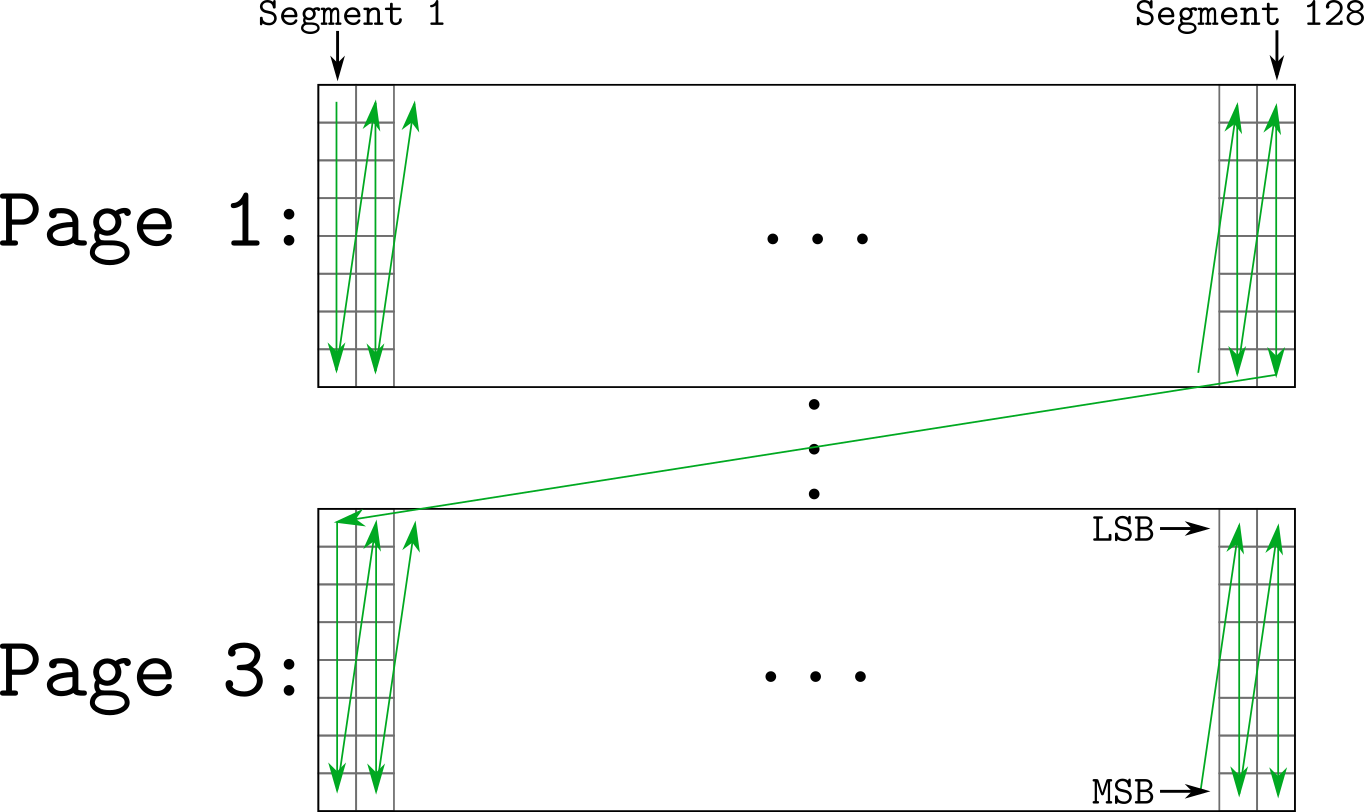
\includegraphics[width=.7\textwidth]{ssd1306}
    \caption{Verarbeitung eines Datenstreams für die Darstellung auf dem Erweiterungsmoduldisplay; abgewandelt von \cite[S.~37]{ssd1306}}
    \label{fig:ssd1306PixelControl}
\end{figure}

Zur Darstellung von Text am Display erfolgt mittels einer Bitmap-Schriftart, da die Art von Schriftarten für eine gute lesbarkeit auf dem kleinen Display optimiert werden kann. Alle Zeichen der Schriftart werden dafür in einem zweidimensionalen Array abgelegt und weisen eine Höhe von 14 und eine Breite von 9 Pixeln auf. Zu Umwandlung von Zeichenketten in Glyphen sind zustätzliche Hilfunktionen implementiert. Die Darstellung von Inhalt auf dem Display erfolgt in zwei Schritten. Im ersten Schritt werden alle Pixelinformationen in einen lokalen Buffer des ESP32 zwischen gespeichert. Der Buffer hat eine Größe von 492~Byte, wo jedes Bit ein Pixel des Displays repräsentiert. Im zweiten Schritt wird der lokale Puffer mittels \ac{I2C} an das Display übertragen und dargestellt. Die Aufteilung in zwei Schritte hat den Vorteil, dass dem ESP32 immer der aktuelle Zustand des Displays bekannt ist und dass das Anzeigen von Elementen am Display einfacher ist, wenn immer der komplette Inhalt des Displays ausgetauscht wird, statt einige Regionen.

\subsection{Kombination aller Softwarekomponenten}
Als Programmiersprache wird C verwendet
%Datenaustausch mittels globale Variablen
    %--> Einen Ablaufbplan hinzufüen, wie neue Daten an das Endgerät weiterversendet werden

%Aufgabenausführung am ESP erklären
    %--> Display wird im Code ausgeführt
    %--> Buttonklick via Interrupts
    %--> BLE Task
    %--> Ermittlung des Spannungslevels mittels ADC und Timer
    %--> Auslesen des CRSF durch Task



\section{Platinenentwurf}
% Schreiben, dass 3 Platinen verwendet wurden, damit die Konstruktion des ersten Prototypen einfacher ist
% Bilder der 3 fertigen Platinen machen
%PCB-Design erklären. (Erklären für was die zonen sind und was beachtet werden musste, batterie auslesen, esd schutz, usb zu serial, schutzschaltung strom, Spannungsregulierung Datenleitungen)
%sektionen des PCB erklären
%schreiben das sich an die Referenzdesing von folgenden Quellen gehalten wurde: Liste von Quellen finden
% Im Anhag die Schematic aller PCBs einfügen.
% ESD Protection durch Dioden am Connector zur Fernsteuerung
% Button sind entprellt --> Beachtet werden muss, dass es an Boot-Button nicht möglich ist, da Kondensator den Pin beim Start auf logisch 0 setzt und dadurch immer beim ersten Starten der Mikrocontroller in Flashmode geht

\section{Gehäuseerstellung}
%besonderheiten des Gehäuses aufzeigen --> im bezug auf 3d druck (Überhänge können nur mit Stützstrukturen gedruckt werden)
    %--> Tasterknopf so hergestellt, dass es in einen Teil mitgedruckt werden kann --> Flexibilät wird erzeugt durch verjüngung der Verbindung zwischen Tastenkopf und Gehäuse
        %--> Bild hinzufügen wie es im inneren Aussieht mit der Verjüngung
        %--> Kone ist dafür noch da damit der tieferliegende Taster ohne zutiefen eindrücken (angenehmes Tastengefühl) betätigt werden kann
    %--> Bild von einen Gewindeeinsatz machen und einfügen --> Wahrscheinlich eher unbekannt
    %--> Aufteilung der unteren hälfte damit diese mit möglichst wenig stütztrukturen auskommt und die qualität des Verbinders zur Fernsteuerung eine gute qualität hat
    %--> Unteres teil kann entweder nur zusammengeschraubt werden, oder empfohlen zu verkleben, damit Teil stabiler ist
    %--> Weiter Halterungen mussten gedruckt werden, da die Connector-Platine sehr nah an der Außenwand des Gehäuse liegt und daher keine Gewindeeinsätze darunter plaziert werden können
%damit platinen und Gehäuse festgeschraubt werden kann, wurden in das Gehäuse gewindeeinsätze eingelegt
%3d cad dateien des gehäuses einfügen --> FSTL verwenden --> Vielleicht alle 3-Objekte übereinander fliegen lassen so wie sie zusammengebaut würden und screenshot dann von der Seite